% %%%%%%%%%%%%%%%%%%%%%%%%%%%%%%%%%%%%%%%%%%%%%%%%%%%%%%%%%%%%%%%%%%%%%%%%%%%%%%%%%%%%%%%%%%%%
% PROBLEM SET LATEX TEMPLATE FILE
% DEFINE DOCUMENT STYLE, LOAD PACKAGES
\documentclass[11pt,notitlepage]{article}\usepackage[]{graphicx}\usepackage[]{color}
%% maxwidth is the original width if it is less than linewidth
%% otherwise use linewidth (to make sure the graphics do not exceed the margin)
\makeatletter
\def\maxwidth{ %
  \ifdim\Gin@nat@width>\linewidth
    \linewidth
  \else
    \Gin@nat@width
  \fi
}
\makeatother

\definecolor{fgcolor}{rgb}{0.345, 0.345, 0.345}
\newcommand{\hlnum}[1]{\textcolor[rgb]{0.686,0.059,0.569}{#1}}%
\newcommand{\hlstr}[1]{\textcolor[rgb]{0.192,0.494,0.8}{#1}}%
\newcommand{\hlcom}[1]{\textcolor[rgb]{0.678,0.584,0.686}{\textit{#1}}}%
\newcommand{\hlopt}[1]{\textcolor[rgb]{0,0,0}{#1}}%
\newcommand{\hlstd}[1]{\textcolor[rgb]{0.345,0.345,0.345}{#1}}%
\newcommand{\hlkwa}[1]{\textcolor[rgb]{0.161,0.373,0.58}{\textbf{#1}}}%
\newcommand{\hlkwb}[1]{\textcolor[rgb]{0.69,0.353,0.396}{#1}}%
\newcommand{\hlkwc}[1]{\textcolor[rgb]{0.333,0.667,0.333}{#1}}%
\newcommand{\hlkwd}[1]{\textcolor[rgb]{0.737,0.353,0.396}{\textbf{#1}}}%

\usepackage{framed}
\makeatletter
\newenvironment{kframe}{%
 \def\at@end@of@kframe{}%
 \ifinner\ifhmode%
  \def\at@end@of@kframe{\end{minipage}}%
  \begin{minipage}{\columnwidth}%
 \fi\fi%
 \def\FrameCommand##1{\hskip\@totalleftmargin \hskip-\fboxsep
 \colorbox{shadecolor}{##1}\hskip-\fboxsep
     % There is no \\@totalrightmargin, so:
     \hskip-\linewidth \hskip-\@totalleftmargin \hskip\columnwidth}%
 \MakeFramed {\advance\hsize-\width
   \@totalleftmargin\z@ \linewidth\hsize
   \@setminipage}}%
 {\par\unskip\endMakeFramed%
 \at@end@of@kframe}
\makeatother

\definecolor{shadecolor}{rgb}{.97, .97, .97}
\definecolor{messagecolor}{rgb}{0, 0, 0}
\definecolor{warningcolor}{rgb}{1, 0, 1}
\definecolor{errorcolor}{rgb}{1, 0, 0}
\newenvironment{knitrout}{}{} % an empty environment to be redefined in TeX

\usepackage{alltt}    % ADD COMMENTS USING A PERCENT SIGN
\usepackage{amsfonts}
\usepackage{amsthm}
\usepackage{amsmath, booktabs}
\usepackage{mathtools}
\usepackage{amssymb}
\usepackage{subfig}
\usepackage{setspace}
\usepackage{fullpage}
\usepackage{verbatim}
\usepackage{graphicx}
\usepackage{tabularx}
\usepackage{longtable}
\usepackage{multicol}
\usepackage{multirow}
\setlength{\parindent}{0in}  	% uncomment to remove indent at start of paragraphs
\usepackage{pdflscape}
\usepackage[english]{babel}
\usepackage[pdftex]{hyperref}
\usepackage{natbib}
\usepackage{caption}
\usepackage{amsmath}
\usepackage{amsfonts}
\usepackage{graphics}
\usepackage{multirow}
\usepackage{graphics}
\usepackage{hyperref}
\usepackage{longtable}
\usepackage{latexsym}
\usepackage{rotating}
\usepackage{setspace}
\usepackage{layouts} 
\usepackage[titletoc]{appendix}
\DeclareGraphicsExtensions{.pdf,.jpg,.png}
\usepackage[margin=1in]{geometry}
\usepackage{enumerate}
\usepackage{float}

\newcolumntype{L}[1]{>{\raggedright\let\newline\\\arraybackslash\hspace{0pt}}m{#1}}
\newcolumntype{C}[1]{>{\centering\let\newline\\\arraybackslash\hspace{0pt}}m{#1}}
\newcolumntype{R}[1]{>{\raggedleft\let\newline\\\arraybackslash\hspace{0pt}}m{#1}}

\usepackage[T1]{fontenc}				

\usepackage{xcolor}
\usepackage[printwatermark]{xwatermark}

\usepackage{textcomp} % defines textquotesingle
 \AtBeginDocument{%
        \def\PYZsq{\textquotesingle}% Upright quotes in Pygmentized code
    }
 
 \usepackage{fancyvrb} % verbatim replacement that allows latex
    % Hack from http://tex.stackexchange.com/a/47451/13684:
    \AtBeginDocument{%
        \def\PYZsq{\textquotesingle}% Upright quotes in Pygmentized code
    }
    \usepackage{upquote} % Upright quotes for verbatim code
 


    % Pygments definitions
    
\makeatletter
\def\PY@reset{\let\PY@it=\relax \let\PY@bf=\relax%
    \let\PY@ul=\relax \let\PY@tc=\relax%
    \let\PY@bc=\relax \let\PY@ff=\relax}
\def\PY@tok#1{\csname PY@tok@#1\endcsname}
\def\PY@toks#1+{\ifx\relax#1\empty\else%
    \PY@tok{#1}\expandafter\PY@toks\fi}
\def\PY@do#1{\PY@bc{\PY@tc{\PY@ul{%
    \PY@it{\PY@bf{\PY@ff{#1}}}}}}}
\def\PY#1#2{\PY@reset\PY@toks#1+\relax+\PY@do{#2}}

\expandafter\def\csname PY@tok@w\endcsname{\def\PY@tc##1{\textcolor[rgb]{0.73,0.73,0.73}{##1}}}
\expandafter\def\csname PY@tok@c\endcsname{\let\PY@it=\textit\def\PY@tc##1{\textcolor[rgb]{0.25,0.50,0.50}{##1}}}
\expandafter\def\csname PY@tok@cp\endcsname{\def\PY@tc##1{\textcolor[rgb]{0.74,0.48,0.00}{##1}}}
\expandafter\def\csname PY@tok@k\endcsname{\let\PY@bf=\textbf\def\PY@tc##1{\textcolor[rgb]{0.00,0.50,0.00}{##1}}}
\expandafter\def\csname PY@tok@kp\endcsname{\def\PY@tc##1{\textcolor[rgb]{0.00,0.50,0.00}{##1}}}
\expandafter\def\csname PY@tok@kt\endcsname{\def\PY@tc##1{\textcolor[rgb]{0.69,0.00,0.25}{##1}}}
\expandafter\def\csname PY@tok@o\endcsname{\def\PY@tc##1{\textcolor[rgb]{0.40,0.40,0.40}{##1}}}
\expandafter\def\csname PY@tok@ow\endcsname{\let\PY@bf=\textbf\def\PY@tc##1{\textcolor[rgb]{0.67,0.13,1.00}{##1}}}
\expandafter\def\csname PY@tok@nb\endcsname{\def\PY@tc##1{\textcolor[rgb]{0.00,0.50,0.00}{##1}}}
\expandafter\def\csname PY@tok@nf\endcsname{\def\PY@tc##1{\textcolor[rgb]{0.00,0.00,1.00}{##1}}}
\expandafter\def\csname PY@tok@nc\endcsname{\let\PY@bf=\textbf\def\PY@tc##1{\textcolor[rgb]{0.00,0.00,1.00}{##1}}}
\expandafter\def\csname PY@tok@nn\endcsname{\let\PY@bf=\textbf\def\PY@tc##1{\textcolor[rgb]{0.00,0.00,1.00}{##1}}}
\expandafter\def\csname PY@tok@ne\endcsname{\let\PY@bf=\textbf\def\PY@tc##1{\textcolor[rgb]{0.82,0.25,0.23}{##1}}}
\expandafter\def\csname PY@tok@nv\endcsname{\def\PY@tc##1{\textcolor[rgb]{0.10,0.09,0.49}{##1}}}
\expandafter\def\csname PY@tok@no\endcsname{\def\PY@tc##1{\textcolor[rgb]{0.53,0.00,0.00}{##1}}}
\expandafter\def\csname PY@tok@nl\endcsname{\def\PY@tc##1{\textcolor[rgb]{0.63,0.63,0.00}{##1}}}
\expandafter\def\csname PY@tok@ni\endcsname{\let\PY@bf=\textbf\def\PY@tc##1{\textcolor[rgb]{0.60,0.60,0.60}{##1}}}
\expandafter\def\csname PY@tok@na\endcsname{\def\PY@tc##1{\textcolor[rgb]{0.49,0.56,0.16}{##1}}}
\expandafter\def\csname PY@tok@nt\endcsname{\let\PY@bf=\textbf\def\PY@tc##1{\textcolor[rgb]{0.00,0.50,0.00}{##1}}}
\expandafter\def\csname PY@tok@nd\endcsname{\def\PY@tc##1{\textcolor[rgb]{0.67,0.13,1.00}{##1}}}
\expandafter\def\csname PY@tok@s\endcsname{\def\PY@tc##1{\textcolor[rgb]{0.73,0.13,0.13}{##1}}}
\expandafter\def\csname PY@tok@sd\endcsname{\let\PY@it=\textit\def\PY@tc##1{\textcolor[rgb]{0.73,0.13,0.13}{##1}}}
\expandafter\def\csname PY@tok@si\endcsname{\let\PY@bf=\textbf\def\PY@tc##1{\textcolor[rgb]{0.73,0.40,0.53}{##1}}}
\expandafter\def\csname PY@tok@se\endcsname{\let\PY@bf=\textbf\def\PY@tc##1{\textcolor[rgb]{0.73,0.40,0.13}{##1}}}
\expandafter\def\csname PY@tok@sr\endcsname{\def\PY@tc##1{\textcolor[rgb]{0.73,0.40,0.53}{##1}}}
\expandafter\def\csname PY@tok@ss\endcsname{\def\PY@tc##1{\textcolor[rgb]{0.10,0.09,0.49}{##1}}}
\expandafter\def\csname PY@tok@sx\endcsname{\def\PY@tc##1{\textcolor[rgb]{0.00,0.50,0.00}{##1}}}
\expandafter\def\csname PY@tok@m\endcsname{\def\PY@tc##1{\textcolor[rgb]{0.40,0.40,0.40}{##1}}}
\expandafter\def\csname PY@tok@gh\endcsname{\let\PY@bf=\textbf\def\PY@tc##1{\textcolor[rgb]{0.00,0.00,0.50}{##1}}}
\expandafter\def\csname PY@tok@gu\endcsname{\let\PY@bf=\textbf\def\PY@tc##1{\textcolor[rgb]{0.50,0.00,0.50}{##1}}}
\expandafter\def\csname PY@tok@gd\endcsname{\def\PY@tc##1{\textcolor[rgb]{0.63,0.00,0.00}{##1}}}
\expandafter\def\csname PY@tok@gi\endcsname{\def\PY@tc##1{\textcolor[rgb]{0.00,0.63,0.00}{##1}}}
\expandafter\def\csname PY@tok@gr\endcsname{\def\PY@tc##1{\textcolor[rgb]{1.00,0.00,0.00}{##1}}}
\expandafter\def\csname PY@tok@ge\endcsname{\let\PY@it=\textit}
\expandafter\def\csname PY@tok@gs\endcsname{\let\PY@bf=\textbf}
\expandafter\def\csname PY@tok@gp\endcsname{\let\PY@bf=\textbf\def\PY@tc##1{\textcolor[rgb]{0.00,0.00,0.50}{##1}}}
\expandafter\def\csname PY@tok@go\endcsname{\def\PY@tc##1{\textcolor[rgb]{0.53,0.53,0.53}{##1}}}
\expandafter\def\csname PY@tok@gt\endcsname{\def\PY@tc##1{\textcolor[rgb]{0.00,0.27,0.87}{##1}}}
\expandafter\def\csname PY@tok@err\endcsname{\def\PY@bc##1{\setlength{\fboxsep}{0pt}\fcolorbox[rgb]{1.00,0.00,0.00}{1,1,1}{\strut ##1}}}
\expandafter\def\csname PY@tok@kc\endcsname{\let\PY@bf=\textbf\def\PY@tc##1{\textcolor[rgb]{0.00,0.50,0.00}{##1}}}
\expandafter\def\csname PY@tok@kd\endcsname{\let\PY@bf=\textbf\def\PY@tc##1{\textcolor[rgb]{0.00,0.50,0.00}{##1}}}
\expandafter\def\csname PY@tok@kn\endcsname{\let\PY@bf=\textbf\def\PY@tc##1{\textcolor[rgb]{0.00,0.50,0.00}{##1}}}
\expandafter\def\csname PY@tok@kr\endcsname{\let\PY@bf=\textbf\def\PY@tc##1{\textcolor[rgb]{0.00,0.50,0.00}{##1}}}
\expandafter\def\csname PY@tok@bp\endcsname{\def\PY@tc##1{\textcolor[rgb]{0.00,0.50,0.00}{##1}}}
\expandafter\def\csname PY@tok@fm\endcsname{\def\PY@tc##1{\textcolor[rgb]{0.00,0.00,1.00}{##1}}}
\expandafter\def\csname PY@tok@vc\endcsname{\def\PY@tc##1{\textcolor[rgb]{0.10,0.09,0.49}{##1}}}
\expandafter\def\csname PY@tok@vg\endcsname{\def\PY@tc##1{\textcolor[rgb]{0.10,0.09,0.49}{##1}}}
\expandafter\def\csname PY@tok@vi\endcsname{\def\PY@tc##1{\textcolor[rgb]{0.10,0.09,0.49}{##1}}}
\expandafter\def\csname PY@tok@vm\endcsname{\def\PY@tc##1{\textcolor[rgb]{0.10,0.09,0.49}{##1}}}
\expandafter\def\csname PY@tok@sa\endcsname{\def\PY@tc##1{\textcolor[rgb]{0.73,0.13,0.13}{##1}}}
\expandafter\def\csname PY@tok@sb\endcsname{\def\PY@tc##1{\textcolor[rgb]{0.73,0.13,0.13}{##1}}}
\expandafter\def\csname PY@tok@sc\endcsname{\def\PY@tc##1{\textcolor[rgb]{0.73,0.13,0.13}{##1}}}
\expandafter\def\csname PY@tok@dl\endcsname{\def\PY@tc##1{\textcolor[rgb]{0.73,0.13,0.13}{##1}}}
\expandafter\def\csname PY@tok@s2\endcsname{\def\PY@tc##1{\textcolor[rgb]{0.73,0.13,0.13}{##1}}}
\expandafter\def\csname PY@tok@sh\endcsname{\def\PY@tc##1{\textcolor[rgb]{0.73,0.13,0.13}{##1}}}
\expandafter\def\csname PY@tok@s1\endcsname{\def\PY@tc##1{\textcolor[rgb]{0.73,0.13,0.13}{##1}}}
\expandafter\def\csname PY@tok@mb\endcsname{\def\PY@tc##1{\textcolor[rgb]{0.40,0.40,0.40}{##1}}}
\expandafter\def\csname PY@tok@mf\endcsname{\def\PY@tc##1{\textcolor[rgb]{0.40,0.40,0.40}{##1}}}
\expandafter\def\csname PY@tok@mh\endcsname{\def\PY@tc##1{\textcolor[rgb]{0.40,0.40,0.40}{##1}}}
\expandafter\def\csname PY@tok@mi\endcsname{\def\PY@tc##1{\textcolor[rgb]{0.40,0.40,0.40}{##1}}}
\expandafter\def\csname PY@tok@il\endcsname{\def\PY@tc##1{\textcolor[rgb]{0.40,0.40,0.40}{##1}}}
\expandafter\def\csname PY@tok@mo\endcsname{\def\PY@tc##1{\textcolor[rgb]{0.40,0.40,0.40}{##1}}}
\expandafter\def\csname PY@tok@ch\endcsname{\let\PY@it=\textit\def\PY@tc##1{\textcolor[rgb]{0.25,0.50,0.50}{##1}}}
\expandafter\def\csname PY@tok@cm\endcsname{\let\PY@it=\textit\def\PY@tc##1{\textcolor[rgb]{0.25,0.50,0.50}{##1}}}
\expandafter\def\csname PY@tok@cpf\endcsname{\let\PY@it=\textit\def\PY@tc##1{\textcolor[rgb]{0.25,0.50,0.50}{##1}}}
\expandafter\def\csname PY@tok@c1\endcsname{\let\PY@it=\textit\def\PY@tc##1{\textcolor[rgb]{0.25,0.50,0.50}{##1}}}
\expandafter\def\csname PY@tok@cs\endcsname{\let\PY@it=\textit\def\PY@tc##1{\textcolor[rgb]{0.25,0.50,0.50}{##1}}}

\def\PYZbs{\char`\\}
\def\PYZus{\char`\_}
\def\PYZob{\char`\{}
\def\PYZcb{\char`\}}
\def\PYZca{\char`\^}
\def\PYZam{\char`\&}
\def\PYZlt{\char`\<}
\def\PYZgt{\char`\>}
\def\PYZsh{\char`\#}
\def\PYZpc{\char`\%}
\def\PYZdl{\char`\$}
\def\PYZhy{\char`\-}
\def\PYZsq{\char`\'}
\def\PYZdq{\char`\"}
\def\PYZti{\char`\~}
% for compatibility with earlier versions
\def\PYZat{@}
\def\PYZlb{[}
\def\PYZrb{]}
\makeatother


    % Exact colors from NB
    \definecolor{incolor}{rgb}{0.0, 0.0, 0.5}
    \definecolor{outcolor}{rgb}{0.545, 0.0, 0.0}
    
    \providecommand{\tightlist}{%
      \setlength{\itemsep}{0pt}\setlength{\parskip}{0pt}}
\DefineVerbatimEnvironment{Highlighting}{Verbatim}{commandchars=\\\{\}}



    




\title{Field Experiments: Design, Analysis and Interpretation \\
Solutions for Chapter 11 Exercises}
\author{Alan S. Gerber and Donald P. Green\footnote{Solutions prepared by Peter M. Aronow and revised by Alexander Coppock}}
\date{\vspace{-5ex}}

%%%%%%%%%%%%%%%%%%%%%%%%%%%%%%%%%%%%%%%%%%%%%%%%%%%%%%%%%%%%%%%%%%%%%%%%%%%%%%%%%%%%%%%%%%%%%
\IfFileExists{upquote.sty}{\usepackage{upquote}}{}
\begin{document}

\maketitle


\section*{Question 1}
Important concepts:
\begin{enumerate}[a)]
\item Explain the distinction between a sample average treatment effect and a population average treatment effect. Why might a researcher be primarily interested in one rather than the other? \\
Answer:\\
Define a population as a set of subjects from which an experimental sample is drawn.Depending on how a sample is drawn, the ATE for the sample may be similar or different from the ATE for the broader population; large, random samples tend to have similar ATEs to their parent populations. Researchers may be interested in the ATE for the sample because their primary goal is to figure out how the subjects in the experiment respond to the treatment. Or researchers may be interested in the ATE for the population because they seek to draw generalizations about how the intervention would work were it applied to others in the population. 

\item What is a meta-analysis? Why is meta-analysis a better way to summarize research findings than comparing the number of studies that show significant estimated treatment effects to the number of studies that show insignificant estimated treatment effects?\\
Answer:\\
Meta-analysis refers to statistical procedures designed to summarize the results of research literatures. Meta-analysis is sometimes described as a ``systematic'' method for constructing a literature review because it summarizes research findings based on a replicable formula. Specifically, when meta-analysis is used to pool several studies, each study's experimental result is weighted according to a formula that follows from an underlying statistical model. In this chapter, the model involves random sampling from a large population, and the formula (fixed effects meta analysis) weights each study to the inverse of its precision, or squared standard error. This procedure is superior to a count of studies that show significant or insignificant results because the latter potentially accords too much weight to small studies that produce statistically insignificant results and too little weight to large studies that convincingly demonstrate an effect when other, smaller studies fail to do so. Another advantage of meta-analysis over this head-count method is that meta-analysis generates a point estimate and confidence interval, which is more informative than a summary statement about statistical significance. 

\item Using equations (11.2), (11.3), and (11.4), provide a hypothetical example to illustrate how uncertainty about the possibility of bias affects the way in which prior beliefs are updated in light of new evidence.\\
Answer:\\
Suppose that a researcher were to conduct a study on the effects of SAT prep classes on SAT scores using an observational design that compares a national random sample of high school seniors who take the class to those who do not. The researcher's normal prior about the ATE is centered at 30 points with a standard deviation of 15 points. The researcher's normal prior about the bias of the design is 15 points with a standard deviation of 10 points. The study's results suggest that the course increases performance by 65 points with a standard deviation of 5 points. In other words, $g=30$, $\sigma^2_g = 225$, $\beta = 15$, $\sigma^2_{\beta} = 100$, $x_e = 65$, and $\sigma^2_{x_e} = 25$. Plugging these numbers into equation (11.3) gives: 

\begin{align*}
\sigma^2_{\bar{\tau}|x_e} = \frac{1}{\frac{1}{\sigma^2_g} + \frac{1}{\sigma^2_{\beta} + \sigma^2_{x_e}}} = \frac{1}{\frac{1}{225} + \frac{1}{100+25}} = 80.36
\end{align*}

Plugging these numbers into equation (11.4) gives: 

\begin{align*}
p_1 &= \frac{\sigma^2_{\bar{\tau}|x_e}}{\sigma^2_g} = \frac{\sigma^2_{\beta} + \sigma^2_{x_e}}{\sigma^2_g +\sigma^2_{\beta} + \sigma^2_{x_e}} = \frac{100+25}{225+100+25} = 0.357
p_2 &= \frac{\sigma^2_{\bar{\tau}|x_e}}{\sigma^2_{\beta} + \sigma^2_{x_e}} = \frac{\sigma^2_g}{\sigma^2_g +\sigma^2_{\beta} + \sigma^2_{x_e}} = 1 - p_1 = 0.643
\end{align*}

Finally, plugging these numbers into equation (11.2) gives the posterior estimate:

\begin{align*}
E[\bar{\tau}|X_e = x_e] &= p_1*g + p_2(x_e - \beta) \\
&= 0.357 * 30 + 0.643*(65-15) = 42.87
\end{align*}

In the absence of uncertainty about bias (i.e., if $\sigma^2_{\beta}=0$), the weight given to the new evidence ($p_2$) would have been much greater: $\frac{\sigma^2_g}{\sigma^2_g +\sigma^2_{\beta} + \sigma^2_{x_e}} = \frac{225}{225 + 0 +25} = 0.9$.  The posterior would have more strongly shaped by the observational results:

\begin{align*}
E[\bar{\tau}|X_e = x_e] &= p_1*g + p_2(x_e - \beta) \\
&= 0.1 * 30 + 0.9*(65-15) = 48
\end{align*}


\item  What does it mean to conduct a hypothesis test that compares two ``nested'' models?\\
Answer:\\
Models are said to be ``nested'' when one model can be written as a special case of another model. For example, if one conducts an experiment with three groups, a control group and two treatments, one could estimate the ATE of each treatment, or one could estimate a nested model in which both treatments are assumed to have the same ATE.  When expressed in regression form (with indicator variables for each treatment), the first model is 
\begin{align*}
Y_i = \beta_0 + \beta_1 D_{1i} + \beta_2 D_{2i} + \epsilon_i
\end{align*}
and the second model is:
\begin{align*}
Y_i = \beta_0 + \beta_1 (D_{1i} + D_{2i}) + \epsilon_i
\end{align*}

\end{enumerate}


\section*{Question 2}
\begin{knitrout}
\definecolor{shadecolor}{rgb}{0.969, 0.969, 0.969}\color{fgcolor}\begin{kframe}
\begin{verbatim}






\end{verbatim}
\end{kframe}
\end{knitrout}


\section*{Question 3}
Suppose one were to sample $N$ subjects at random from a population of $N*$ people. An experiment is performed whereby $m$ of the $N$ subjects are assigned to receive a treatment, and the remaining $N - m$ are assigned to the control group. Suppose that sometime after the treatment is administered, outcomes are measured for all $N*$ people.

\begin{enumerate}[a)]
\item Suppose one estimates the population ATE by comparing the mean outcome among the m subjects in the treatment group to the mean outcome among the $N^* - m$ subjects who were not assigned to the treatment. Is this estimator unbiased?\\
Answer:\\
Yes. The subjects assigned to the treatment and control groups are each random samples from the pool of $N^*$ subjects in the population.  Therefore, they have the same expected potential outcomes.
\item Would the appropriate standard error of this difference-in-means estimator be equation (11.1), equation (3.4), or neither?\\
Answer:\\
The correct formula is a modified version of equation (3.4) in which $N^*$ replaces $N$.
\end{enumerate}


\section*{Question 4}
\begin{knitrout}
\definecolor{shadecolor}{rgb}{0.969, 0.969, 0.969}\color{fgcolor}\begin{kframe}
\begin{verbatim}






\end{verbatim}
\end{kframe}
\end{knitrout}


\section*{Question 5}
Using the Bayesian updating equations, show algebraically how the priors represented in Figure 11.1 combine with the experimental results depicted in order to form a posterior distribution with a mean of 8 and a standard deviation of 0.89.\\
Answer:\\
In this example, $g=0$, $\sigma^2_g = 4$, $\beta = 0$, $\sigma^2_{\beta} = 0$, $x_e = 10$, and $\sigma^2_{x_e} = 1$

Plugging these numbers into equation (11.3) gives: 

 \begin{align*}
\sigma^2_{\bar{\tau}|x_e} = \frac{1}{\frac{1}{\sigma^2_g} + \frac{1}{\sigma^2_{\beta} + \sigma^2_{x_e}}} = \frac{1}{\frac{1}{4} + \frac{1}{0+1}} = 0.8
\end{align*}
 
Plugging these numbers into equation (11.4) gives: 

\begin{align*}
p_1 &= \frac{\sigma^2_{\bar{\tau}|x_e}}{\sigma^2_g} = \frac{\sigma^2_{\beta} + \sigma^2_{x_e}}{\sigma^2_g +\sigma^2_{\beta} + \sigma^2_{x_e}} = \frac{0+1}{4+0+1} = 0.2\\
p_2 &= \frac{\sigma^2_{\bar{\tau}|x_e}}{\sigma^2_{\beta} + \sigma^2_{x_e}} = \frac{\sigma^2_g}{\sigma^2_g +\sigma^2_{\beta} + \sigma^2_{x_e}} = 1 - p_1 = 0.8
\end{align*}

Finally, plugging these numbers into equation (11.2) gives the posterior estimate:

\begin{align*}
E[\bar{\tau}|X_e = x_e] &= p_1*g + p_2(x_e - \beta) \\
&= 0.2 * 0 + 0.8*(10) = 8
\end{align*}

Thus, Figure 11.1 depicts the posterior as centered at 8 with a standard error of $\sqrt{0.8}=0.89$.

\section*{Question 6}
\begin{knitrout}
\definecolor{shadecolor}{rgb}{0.969, 0.969, 0.969}\color{fgcolor}\begin{kframe}
\begin{verbatim}






\end{verbatim}
\end{kframe}
\end{knitrout}


\section*{Question 7}
According to the logistic regression coefficients reported in Table 11.2, the intercept in Region 1 is 8.531 and the slope is -1.978. Based on these numbers, what proportion of those offered a price of 100 shillings is expected to buy a bed net? How does this compare to the actual rate of purchases at this price?\\
Answer:\\
The logistic model for Region 1 is 
\begin{align*}
Pr[Y_i=1] &= \frac{1}{1+e^{-(\beta_0 + \beta_1 ln[D-i])}}\\
&= \frac{1}{1+e^{-(\beta_0 + \beta_1 ln[100])}}\\
&=0.359
\end{align*}
The corresponding empirical value from this region is 0.340.


\section*{Question 8}
\begin{knitrout}
\definecolor{shadecolor}{rgb}{0.969, 0.969, 0.969}\color{fgcolor}\begin{kframe}
\begin{verbatim}






\end{verbatim}
\end{kframe}
\end{knitrout}

\section*{Question 9}
Because the log transformation of price is undefined when price is zero, we excluded the zero price condition from the analysis of bed net purchases in Tables 11.2 and 11.3.

\begin{enumerate}[a)]
\item If we exclude zero prices from our experimental analysis, will our estimate of the causal effect of price be biased?\\
Answer:\\
No. The exclusion is based on the treatment not on the results. Because those receiving the zero price are a random subset of all subjects, excluding these observations does not lead to biased estimates of the ATE. Thinking back to Chapter 7, missingness here is unrelated to potential outcomes.

\item Suppose we reasoned that a nominal price of zero nevertheless involves some transaction cost, as villagers have to make the effort to redeem their vouchers. For a given subject, we may model the probability of making a purchase as:

\begin{equation*}
Pr[Y=1] = \frac{1}{1 + e^{-(\beta_0+\beta_1 ln[V_i+\gamma])}}
\end{equation*}

where $\gamma$ represents the transaction cost of redeeming the voucher. In order to estimate $\gamma$, insert a positive value of $\gamma$, and use logistic regression to estimate the revised model; note the value of the log-likelihood for this model. Repeat this exercise for different values of $\gamma$. Obtain the ``maximum likelihood estimate'' of $\gamma$ by finding the value of $\gamma$ that maximizes the log-likelihood. \\
Answer:\\
We tried different values of $\gamma$ until we came upon the value 19, which maximized the log-likelihood:
\begin{knitrout}
\definecolor{shadecolor}{rgb}{0.969, 0.969, 0.969}\color{fgcolor}\begin{kframe}
    \begin{Verbatim}[commandchars=\\\{\}]
{\color{incolor}In [{\color{incolor}1}]:} import delim .\PY{o}{/}data\PY{o}{/}chapter11\PY{o}{/}Chapter\PYZus{}11\PYZus{}Dupas\PYZus{}2010\PYZus{}Dataset,clear
\end{Verbatim}

    \begin{Verbatim}[commandchars=\\\{\}]
{\color{incolor}In [{\color{incolor}2}]:} \PY{k}{gen} purchased =.
        \PY{k}{replace} purchased = \PY{l+m}{1}\PY{k}{ if} purchasednet\PY{o}{==}\PY{l+s}{\PYZdq{}}\PY{l+s}{y}\PY{l+s}{e}\PY{l+s}{s}\PY{l+s}{\PYZdq{}}
        \PY{k}{replace} purchased = \PY{l+m}{0}\PY{k}{ if} purchasednet\PY{o}{==}\PY{l+s}{\PYZdq{}}\PY{l+s}{n}\PY{l+s}{o}\PY{l+s}{\PYZdq{}}    
        \PY{k}{rename} cfw\PYZus{}id region		
            
        \PY{k}{matrix} t=\PY{n+nf}{J}(\PY{l+m}{100}, \PY{l+m}{2}, .)
        \PY{k}{matrix} colnames t=gammas lls
            
        \PY{k}{forvalues} i = \PY{l+m}{1}\PY{o}{/}\PY{l+m}{100} \PYZob{}
        \PY{k}{		}
        \PY{k}{		gen} log\PYZus{}price\PYZus{}star\PYZus{}\PY{n+nv}{`}\PY{n+nv}{i}\PY{n+nv}{\PYZsq{}} =\PY{k}{ log}(price \PY{o}{+} \PY{n+nv}{`}\PY{n+nv}{i}\PY{n+nv}{\PYZsq{}})
        \PY{k}{		qui}\PY{k}{ glm} purchased log\PYZus{}price\PYZus{}star\PYZus{}\PY{n+nv}{`}\PY{n+nv}{i}\PY{n+nv}{\PYZsq{}} i\PY{l+m}{.}region, 
        			family(binomial) link(logit)
        \PY{k}{		}
        \PY{k}{		matrix} t[\PY{n+nv}{`}\PY{n+nv}{i}\PY{n+nv}{\PYZsq{}}, \PY{l+m}{1}] = \PY{n+nv}{`}\PY{n+nv}{i}\PY{n+nv}{\PYZsq{}}
        \PY{k}{		matrix} t[\PY{n+nv}{`}\PY{n+nv}{i}\PY{n+nv}{\PYZsq{}}, \PY{l+m}{2}] = \PY{n+nv}{`}\PY{n+nv}{e}\PY{n+nv}{(}\PY{n+nv}{l}\PY{n+nv}{l}\PY{n+nv}{)}\PY{n+nv}{\PYZsq{}}
        
        \PYZcb{}
\end{Verbatim}

    \begin{Verbatim}[commandchars=\\\{\}]
{\color{incolor}In [{\color{incolor}3}]:} \PY{k}{svmat} double t, names(col)     
        \PY{k}{qui}\PY{k}{ sum} lls
        \PY{k}{list} gammas\PY{k}{ if} lls\PY{o}{==}\PY{n+nf}{r}(max)
           
        \PY{k}{scatter} lls gammas, xline(\PY{l+m}{19})
        \PY{k}{graph} export ..\PY{o}{/}results\PY{o}{/}chapter11\PY{o}{/}exercise\PYZus{}11\PYZus{}9\PYZus{}graph\PY{l+m}{.}pdf
\end{Verbatim}

    \begin{Verbatim}[commandchars=\\\{\}]
      +--------+
      | gammas |
      |--------|
  19. |     19 |
      +--------+

    \end{Verbatim}
\end{kframe}

{\centering 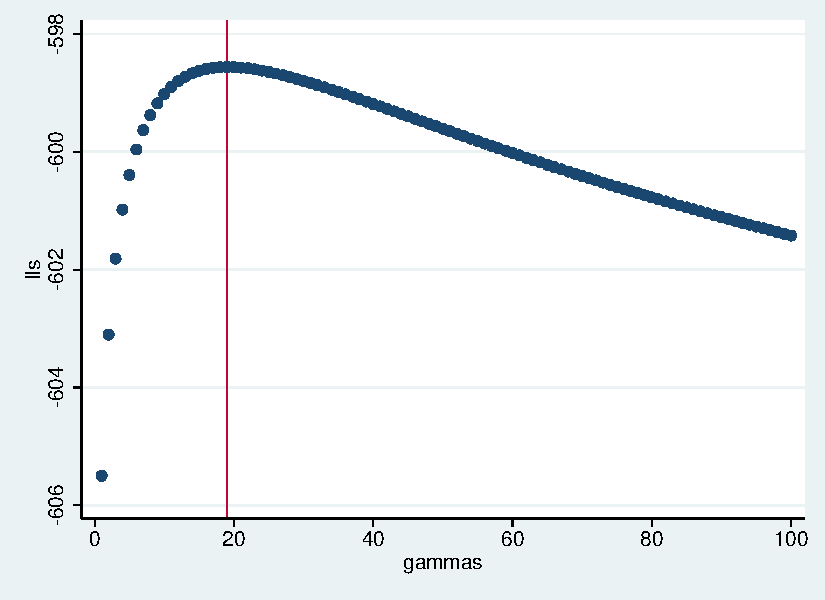
\includegraphics[width=3.7in,height=2.8in]{figure/PS11-unnamed-chunk-6-1} 

}



\end{knitrout}


\item What is the substantive interpretation of the maximum likelihood estimates of $\gamma$ and $\beta_1$? (Note that the standard errors using this method understate the true sampling variability because they are conditional on a particular choice of $\gamma$. Ignore the reported standard errors, and just interpret the estimates.)\\
Answer:\\
The maximum likelihood estimate of $\gamma$ is 19 shillings, which suggests that redeeming the voucher involves some transaction cost even when the nominal price is very small.  The coefficient on the treatment variable, $ln(price+19)$, is -1.98, which suggests that for every one unit change in this rescaled version of the treatment, the log-odds of purchase declines by -1.98.  For example, suppose that the offer price rises from 0 to 100 shillings.  The $ln(price+19)$ would change from 2.94 to 4.78, and this change would reduce the log-odds of purchase by 3.63.To illustrate what this means in terms of percentage points, suppose that a person has a 50\% chance of making a purchase at a price of zero (50\% implies a log-odds of 0). If that person were to be offered a price of 100, the predicted probability of a purchase is $1/(1+e^(-3.63) )=0.026$, or 2.6\%. 


\end{enumerate}
\section*{Question 10}
\begin{knitrout}
\definecolor{shadecolor}{rgb}{0.969, 0.969, 0.969}\color{fgcolor}\begin{kframe}
\begin{verbatim}






\end{verbatim}
\end{kframe}
\end{knitrout}



\end{document}

